\documentclass[../../main.tex]{subfiles}

 \lhead{Implementation: Room Modelling}
 
\begin{document}
\section{Implementation}
	This section describes the steps taken from setting the project objectives to reaching the final implementation of the desired system.


	\subsection{Room Modelling}

		\subsubsection{Room Measurements}

			Before taking room measurements, a quick top-down map of the room was made, highlighting objects, wall indents or protrusions and where doors and windows existed. The dimensions of the room were then measured in meters and noted on the not to scale room map. The tool used for measurements was a DeWalt laser distance measurer \cite{dewalt}. This allowed for accurate measurements of distances that would otherwise not be accessible such as the distance between roof lighting and other fixtures. Once the basic layout had been mapped, maps of individual walls were made and features such as window and door dimensions, distanced between doors etc were noted. The example of an annotated blueprint can be seen in figure~\ref{blueprintTop} in Appendix \ref{appendixA}.

			Hendrix Hall measured at approximately 18.3m x 18.2m x 5.5m.

		\subsubsection{Designing the room}
			\label{designRoom}
			The blue prints were used to model the room in Google SketchUp starting with a hollow rectangle with the dimensions of Hendrix Hall. From this the wall indents and protrusions were modelled by using a push/pull tool. Figure~\ref{sku1} shows an early iteration of the SketchUp model where several wall protrusions have been modelled.

			%-------------Early SketchUp Model Image-------------%
			\begin{figure}[ht]
				\center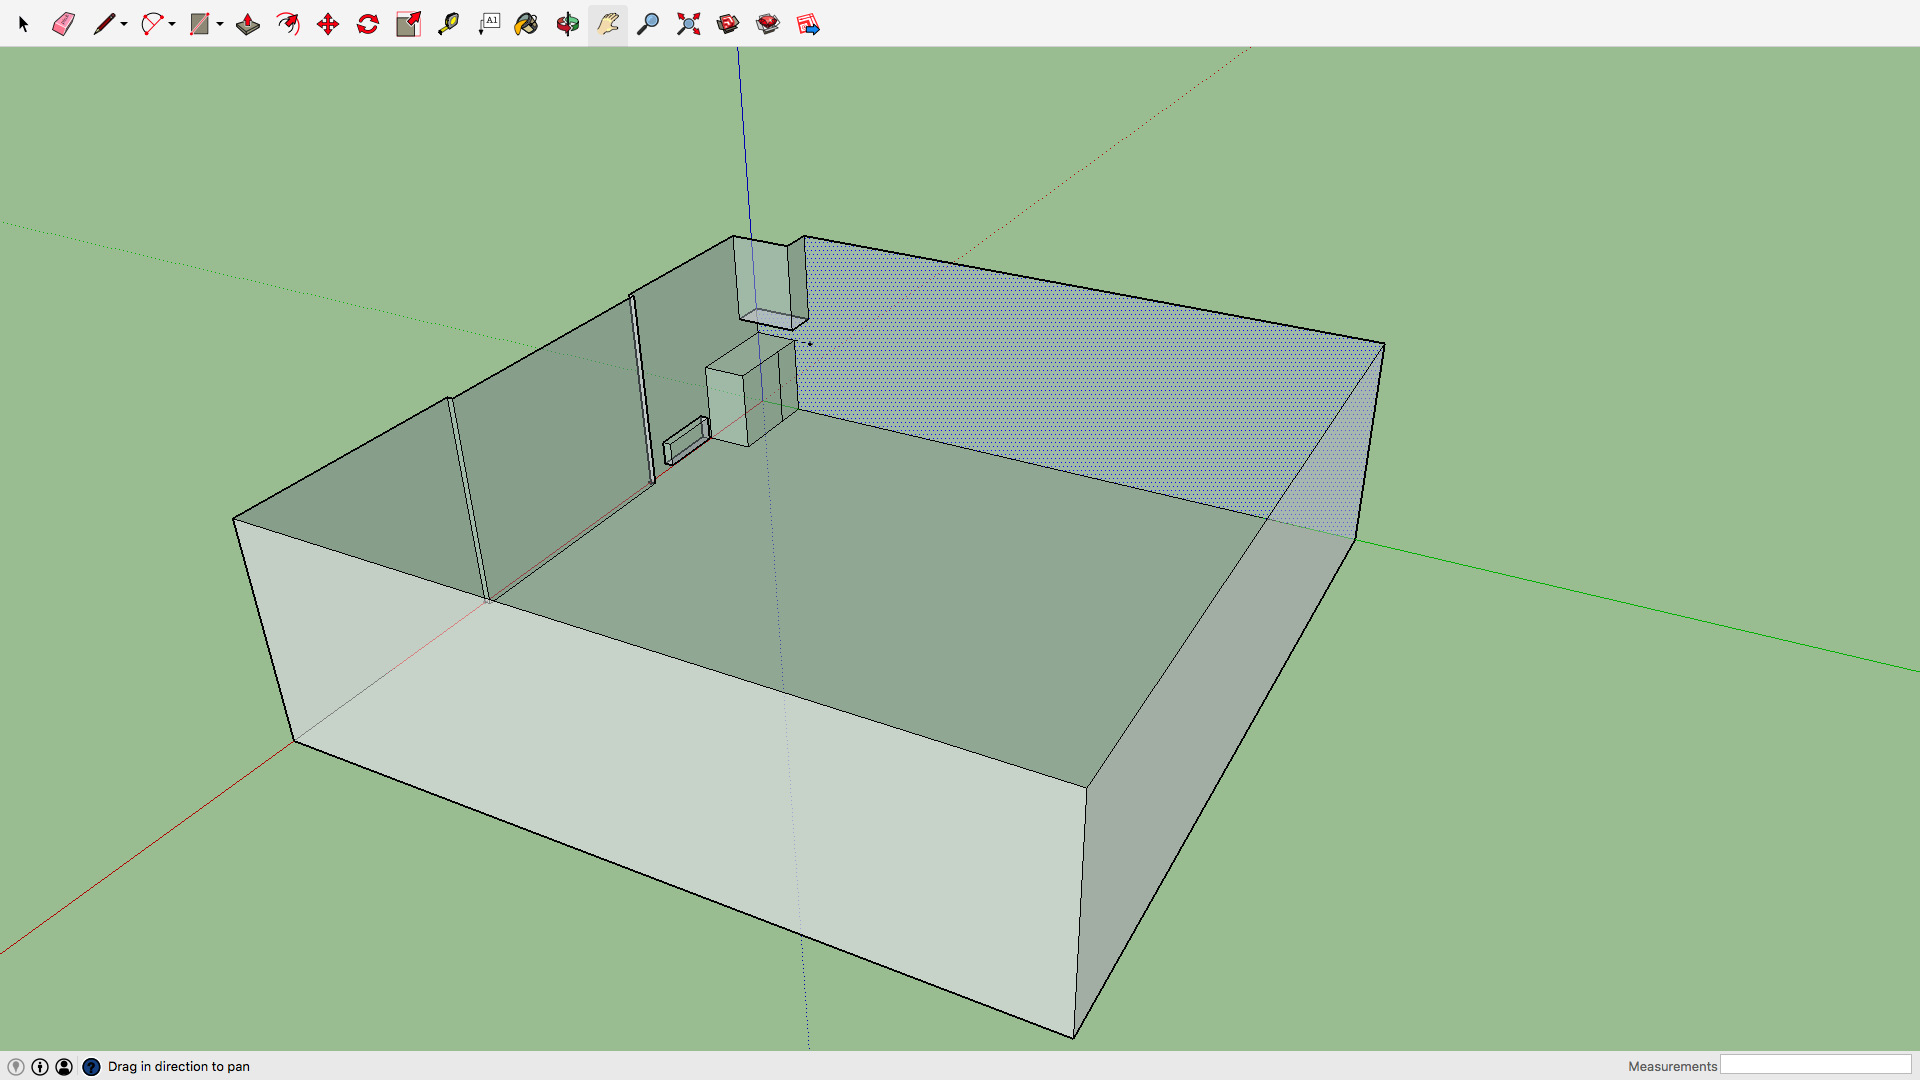
\includegraphics[scale = 0.2]{Sections/Implementation/Modelling/images/sku1.png}
				\caption{Early iteration of the Hendrix Hall SketchUp model with a few early wall protrusions being modelled such as the entrance door}
				\label{sku1}
			\end{figure}

			The contents of Hendrix Hall are predominantly flat surfaces though some more complex surfaces include:

			\begin{itemize}
				\item[-] Lights (concave curves) 
				\item[-] Canvas roof hangings (convex curves) 
				\item[-] Projector hangings (poles)
				%\item[-] Roof (tiled) 
				\item[-] Radiator, door and vent grills \\
			\end{itemize}

			These objects were initially designed to look as close to the real thing as possible, however the objects with curved edges posed a problem when importing the model into Odeon. This is because SketchUp uses a large number of short surfaces to represent curves as can be seen in Figure~\ref{surfaces} which shows the initial models of the lights, projectors and roof hangings. According to the Odeon manual \cite{odeonManual}, when modelling a room for acoustic simulation purposes it is more accurate and less time consuming to keep the model simple and to add the appropriate scattering coefficients or materials in Odeon itself. This also applied to the objects (such as the radiators) that contained a grilled surface, as a specific `grill' material could be selected from Odeons material list (see section \nameref{odeon:materials}).

			%Initially, the more complex surfaces such as the lights, projectors and canvases on the roof were modelled to closely represent those within Hendrix Hall. This resulted in using a large number of individual surfaces to represent the objects curves which can be seen in figure~\ref{surfaces}. Once the model was imported into Odeon this resulted in a large number of surfaces for which materials must be selected for. According to the Odeon manual \cite{odeonManual}, when modelling a room for acoustic simulation purposes it is more accurate and less time consuming to keep the model simple and to add the appropriate scattering coefficients or materials in Odeon itself.

			These objects, shown in figure~\ref{simpleSurfaces} were then redesigned more simply where the roof hangings were represented as four joint slanting surfaces and lights and projector poles are simple rectangles.

			%-------------Lights and projector images-------------%

			\begin{figure}[ht]
				\begin{subfigure}[t]{4in}
					\centering
					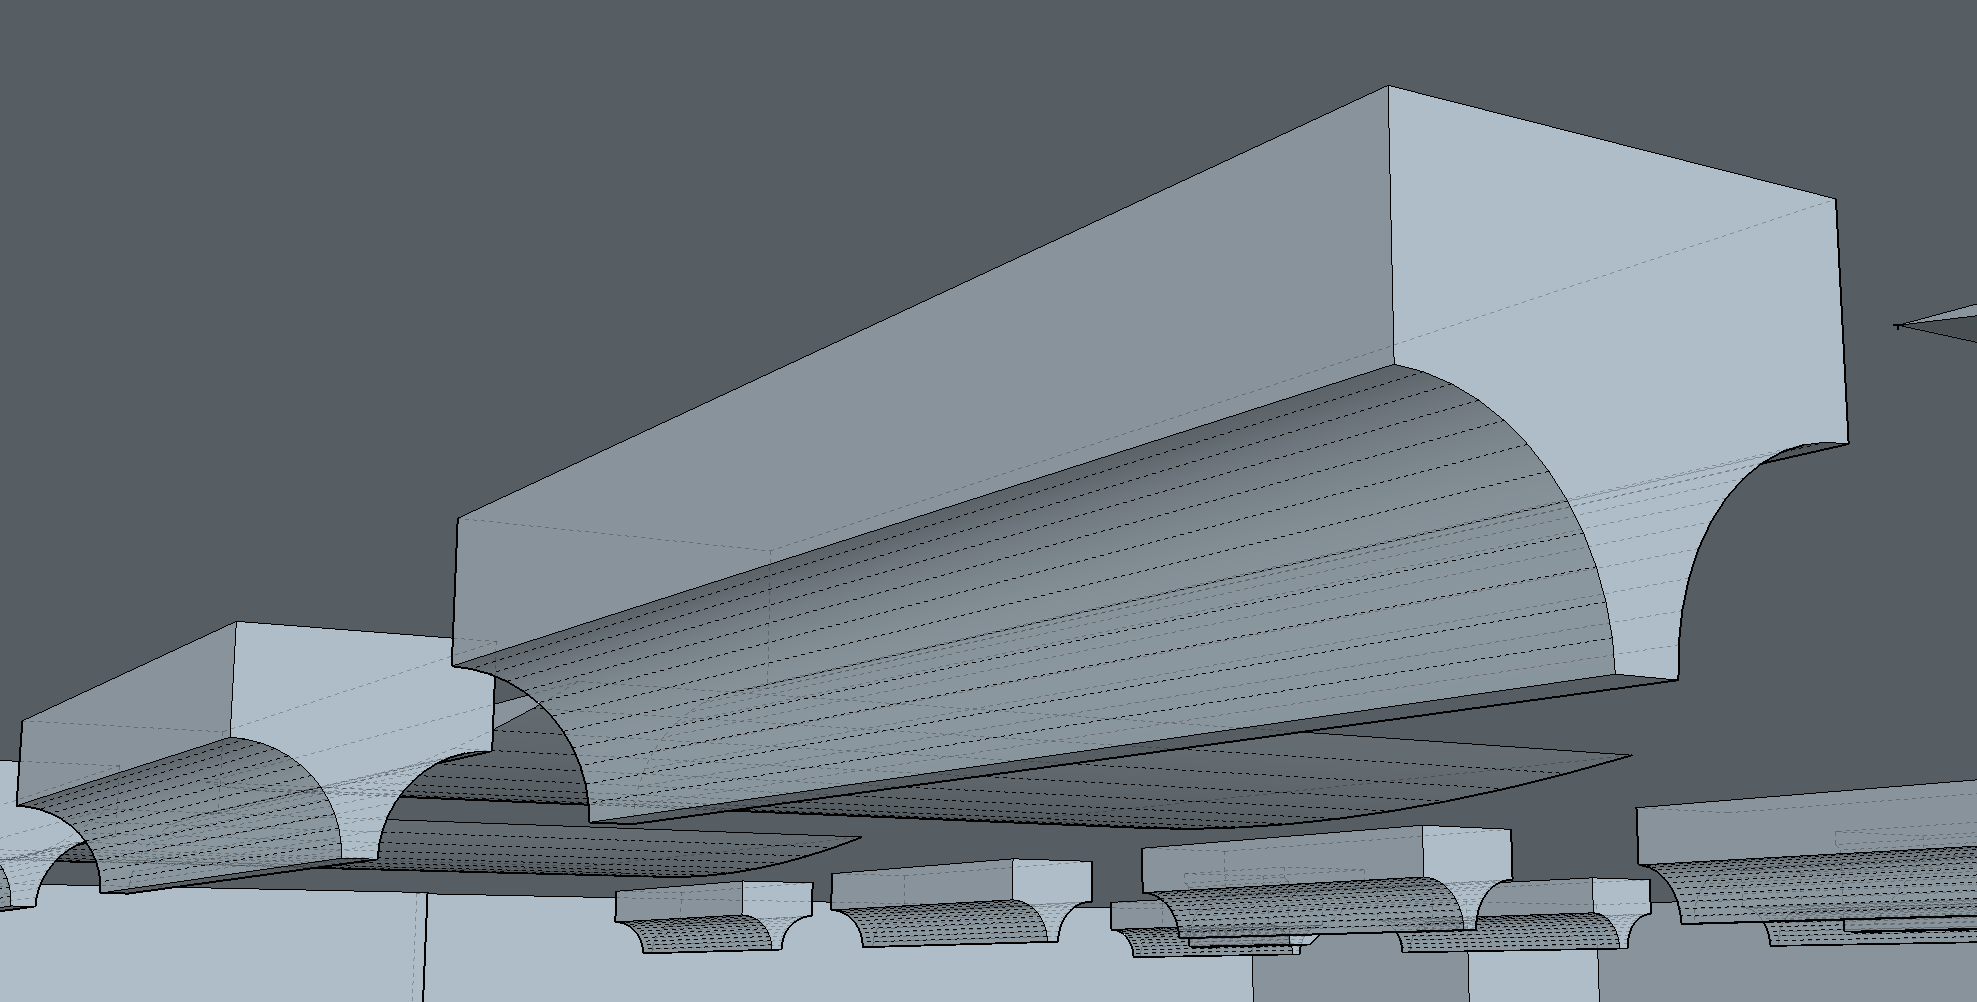
\includegraphics[scale = 0.25]{Sections/Implementation/Modelling/images/lights2.png}
					\caption{Lights}
				\end{subfigure}
				\begin{subfigure}[t]{3in}
					\centering
					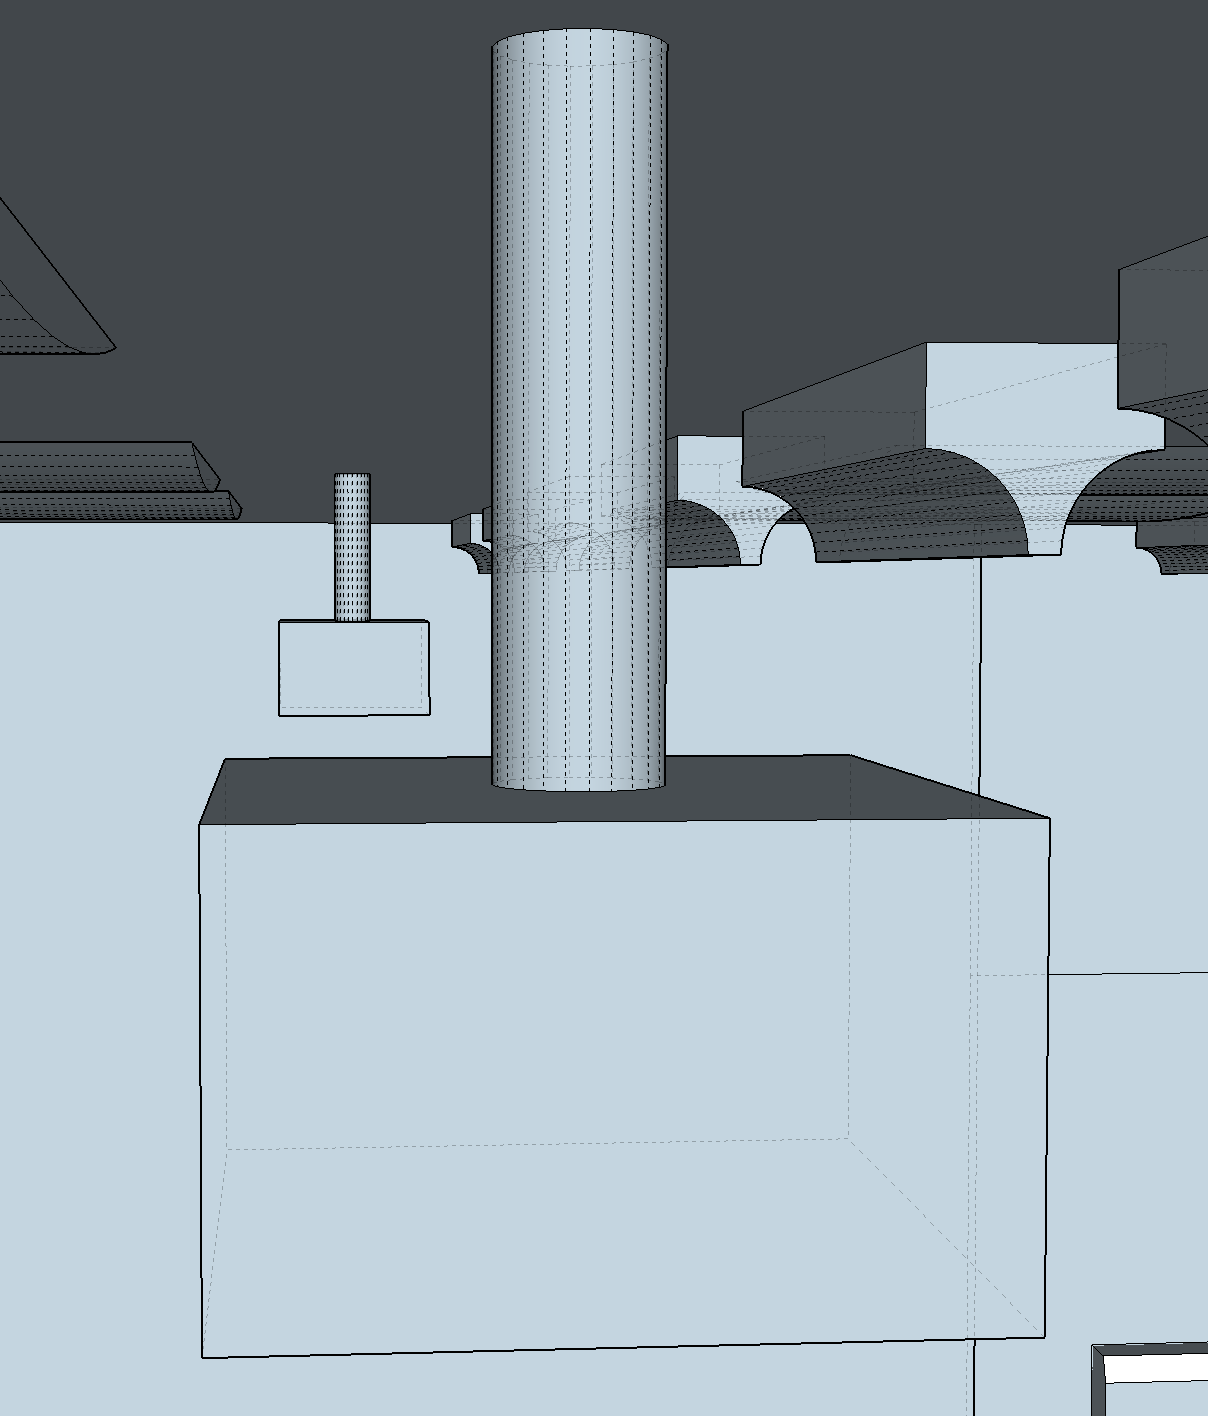
\includegraphics[scale = 0.25]{Sections/Implementation/Modelling/images/projector1.png}
					\caption{Projector}
				\end{subfigure}
				\begin{subfigure}[t]{3in}
					\centering
					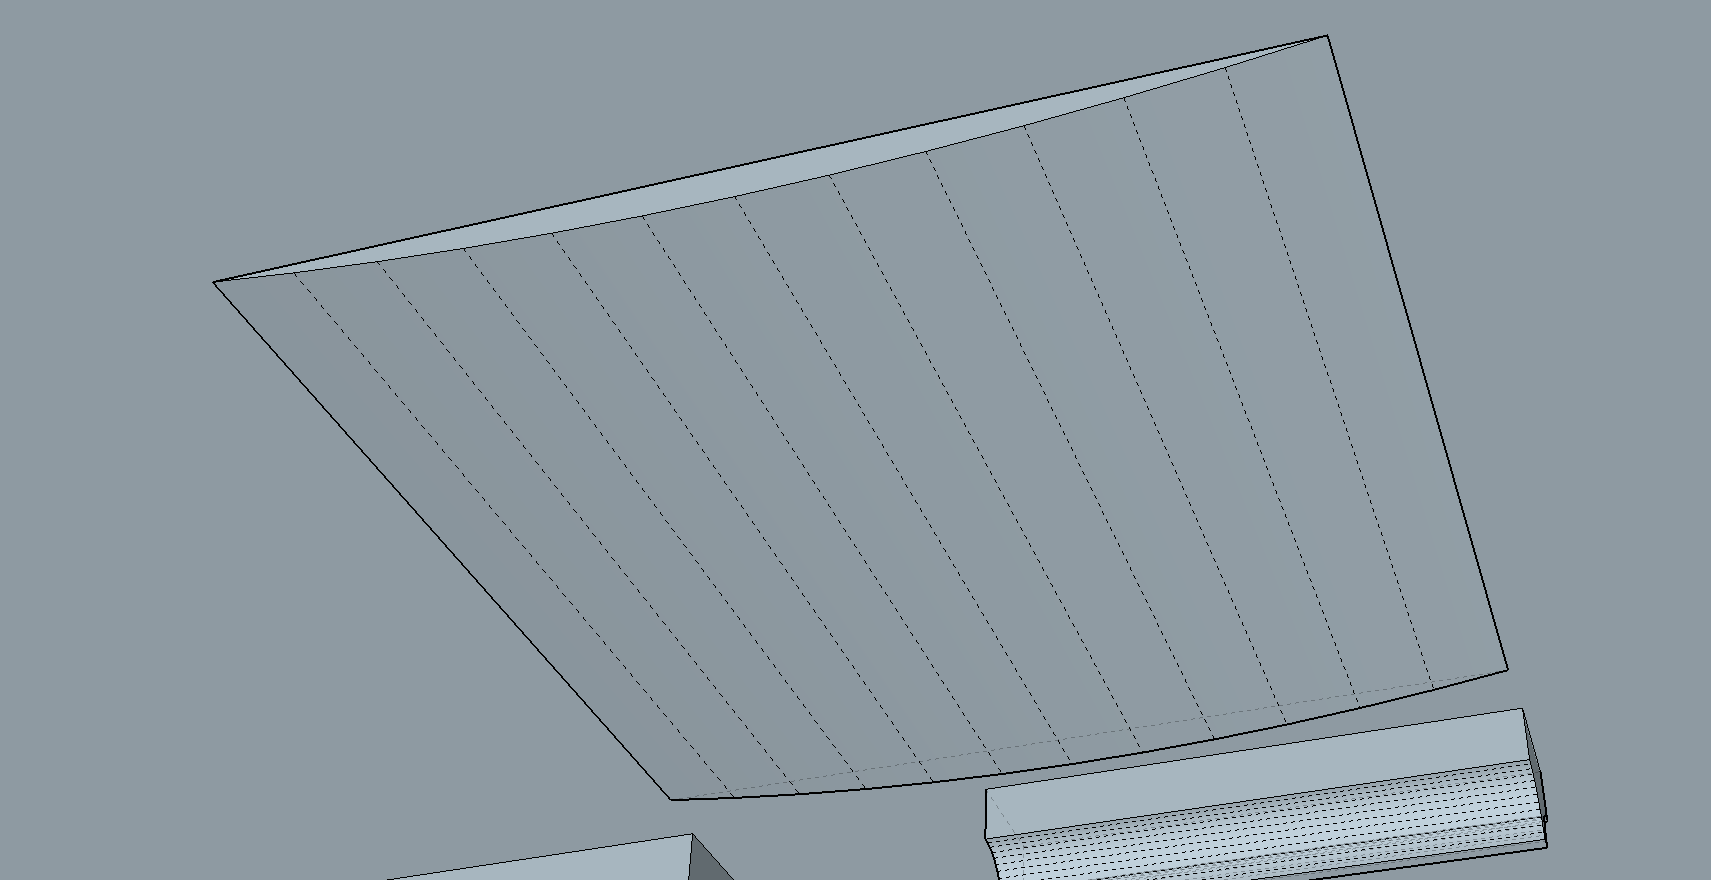
\includegraphics[scale = 0.25]{Sections/Implementation/Modelling/images/concave1.png}
					\caption{Roof Hanging}
				\end{subfigure}
				\caption{Initial models of the lights and projector hangings made of a large number of surfaces}
				\label{surfaces}
			\end{figure}

				%-------------Lights and projector images-------------%

			\begin{figure}[ht]
				\begin{subfigure}[t]{4in}
					\centering
					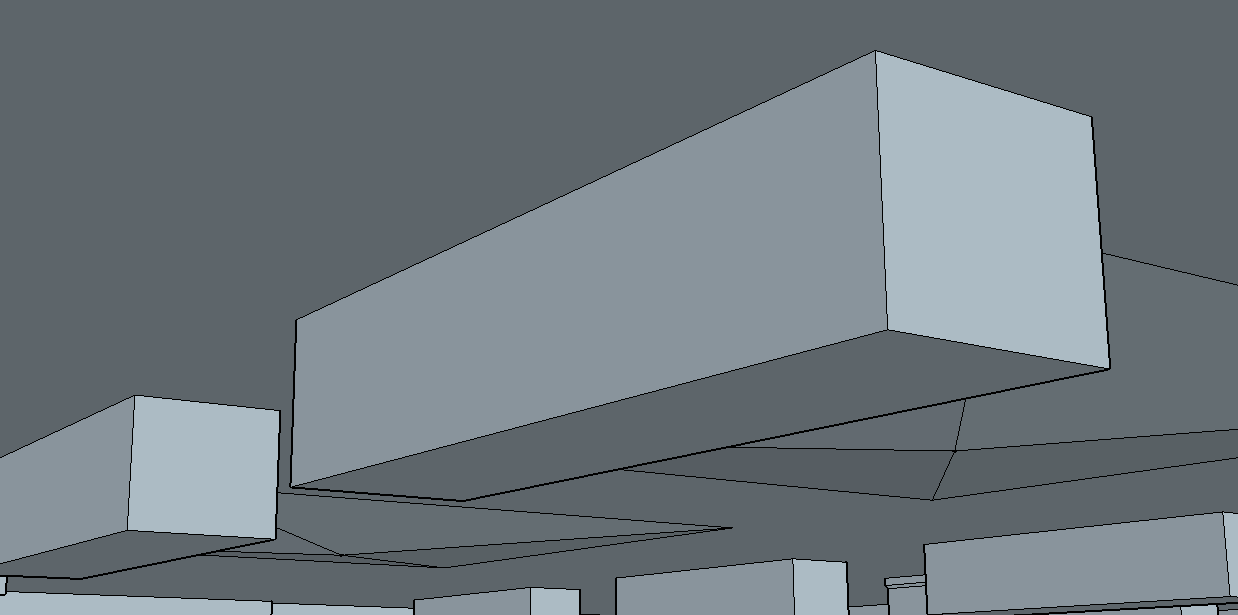
\includegraphics[scale = 0.25]{Sections/Implementation/Modelling/images/lightsSimple.png}
					\caption{Simple Lights}
				\end{subfigure}
				\begin{subfigure}[t]{3in}
					\centering
					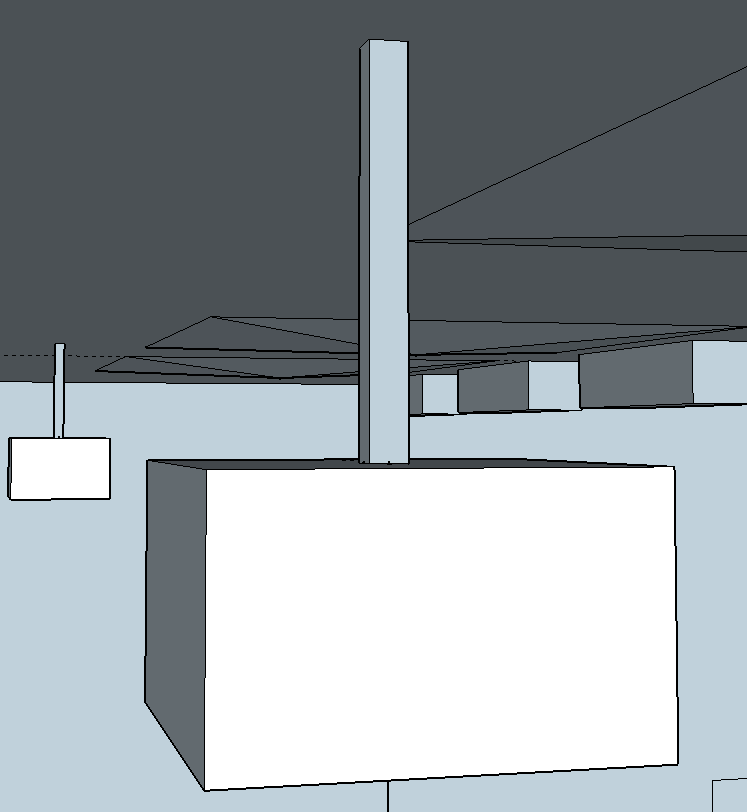
\includegraphics[scale = 0.25]{Sections/Implementation/Modelling/images/projectorSimple.png}
					\caption{Simple Projector}
				\end{subfigure}
				\begin{subfigure}[t]{3in}
					\centering
					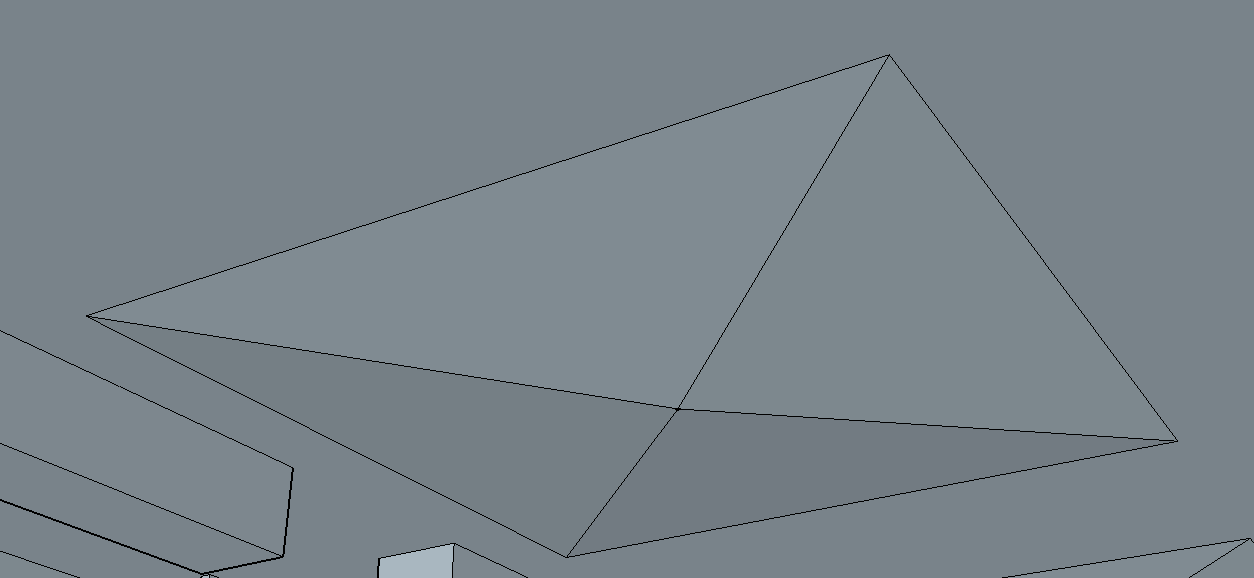
\includegraphics[scale = 0.25]{Sections/Implementation/Modelling/images/concaveSimple.png}
					\caption{Simple Roof Hanging}
				\end{subfigure}
				\caption{Simplified models of the lights and projector hangings containing a smaller number of surfaces}
				\label{simpleSurfaces}
			\end{figure}

		\begin{figure}[ht]
				\center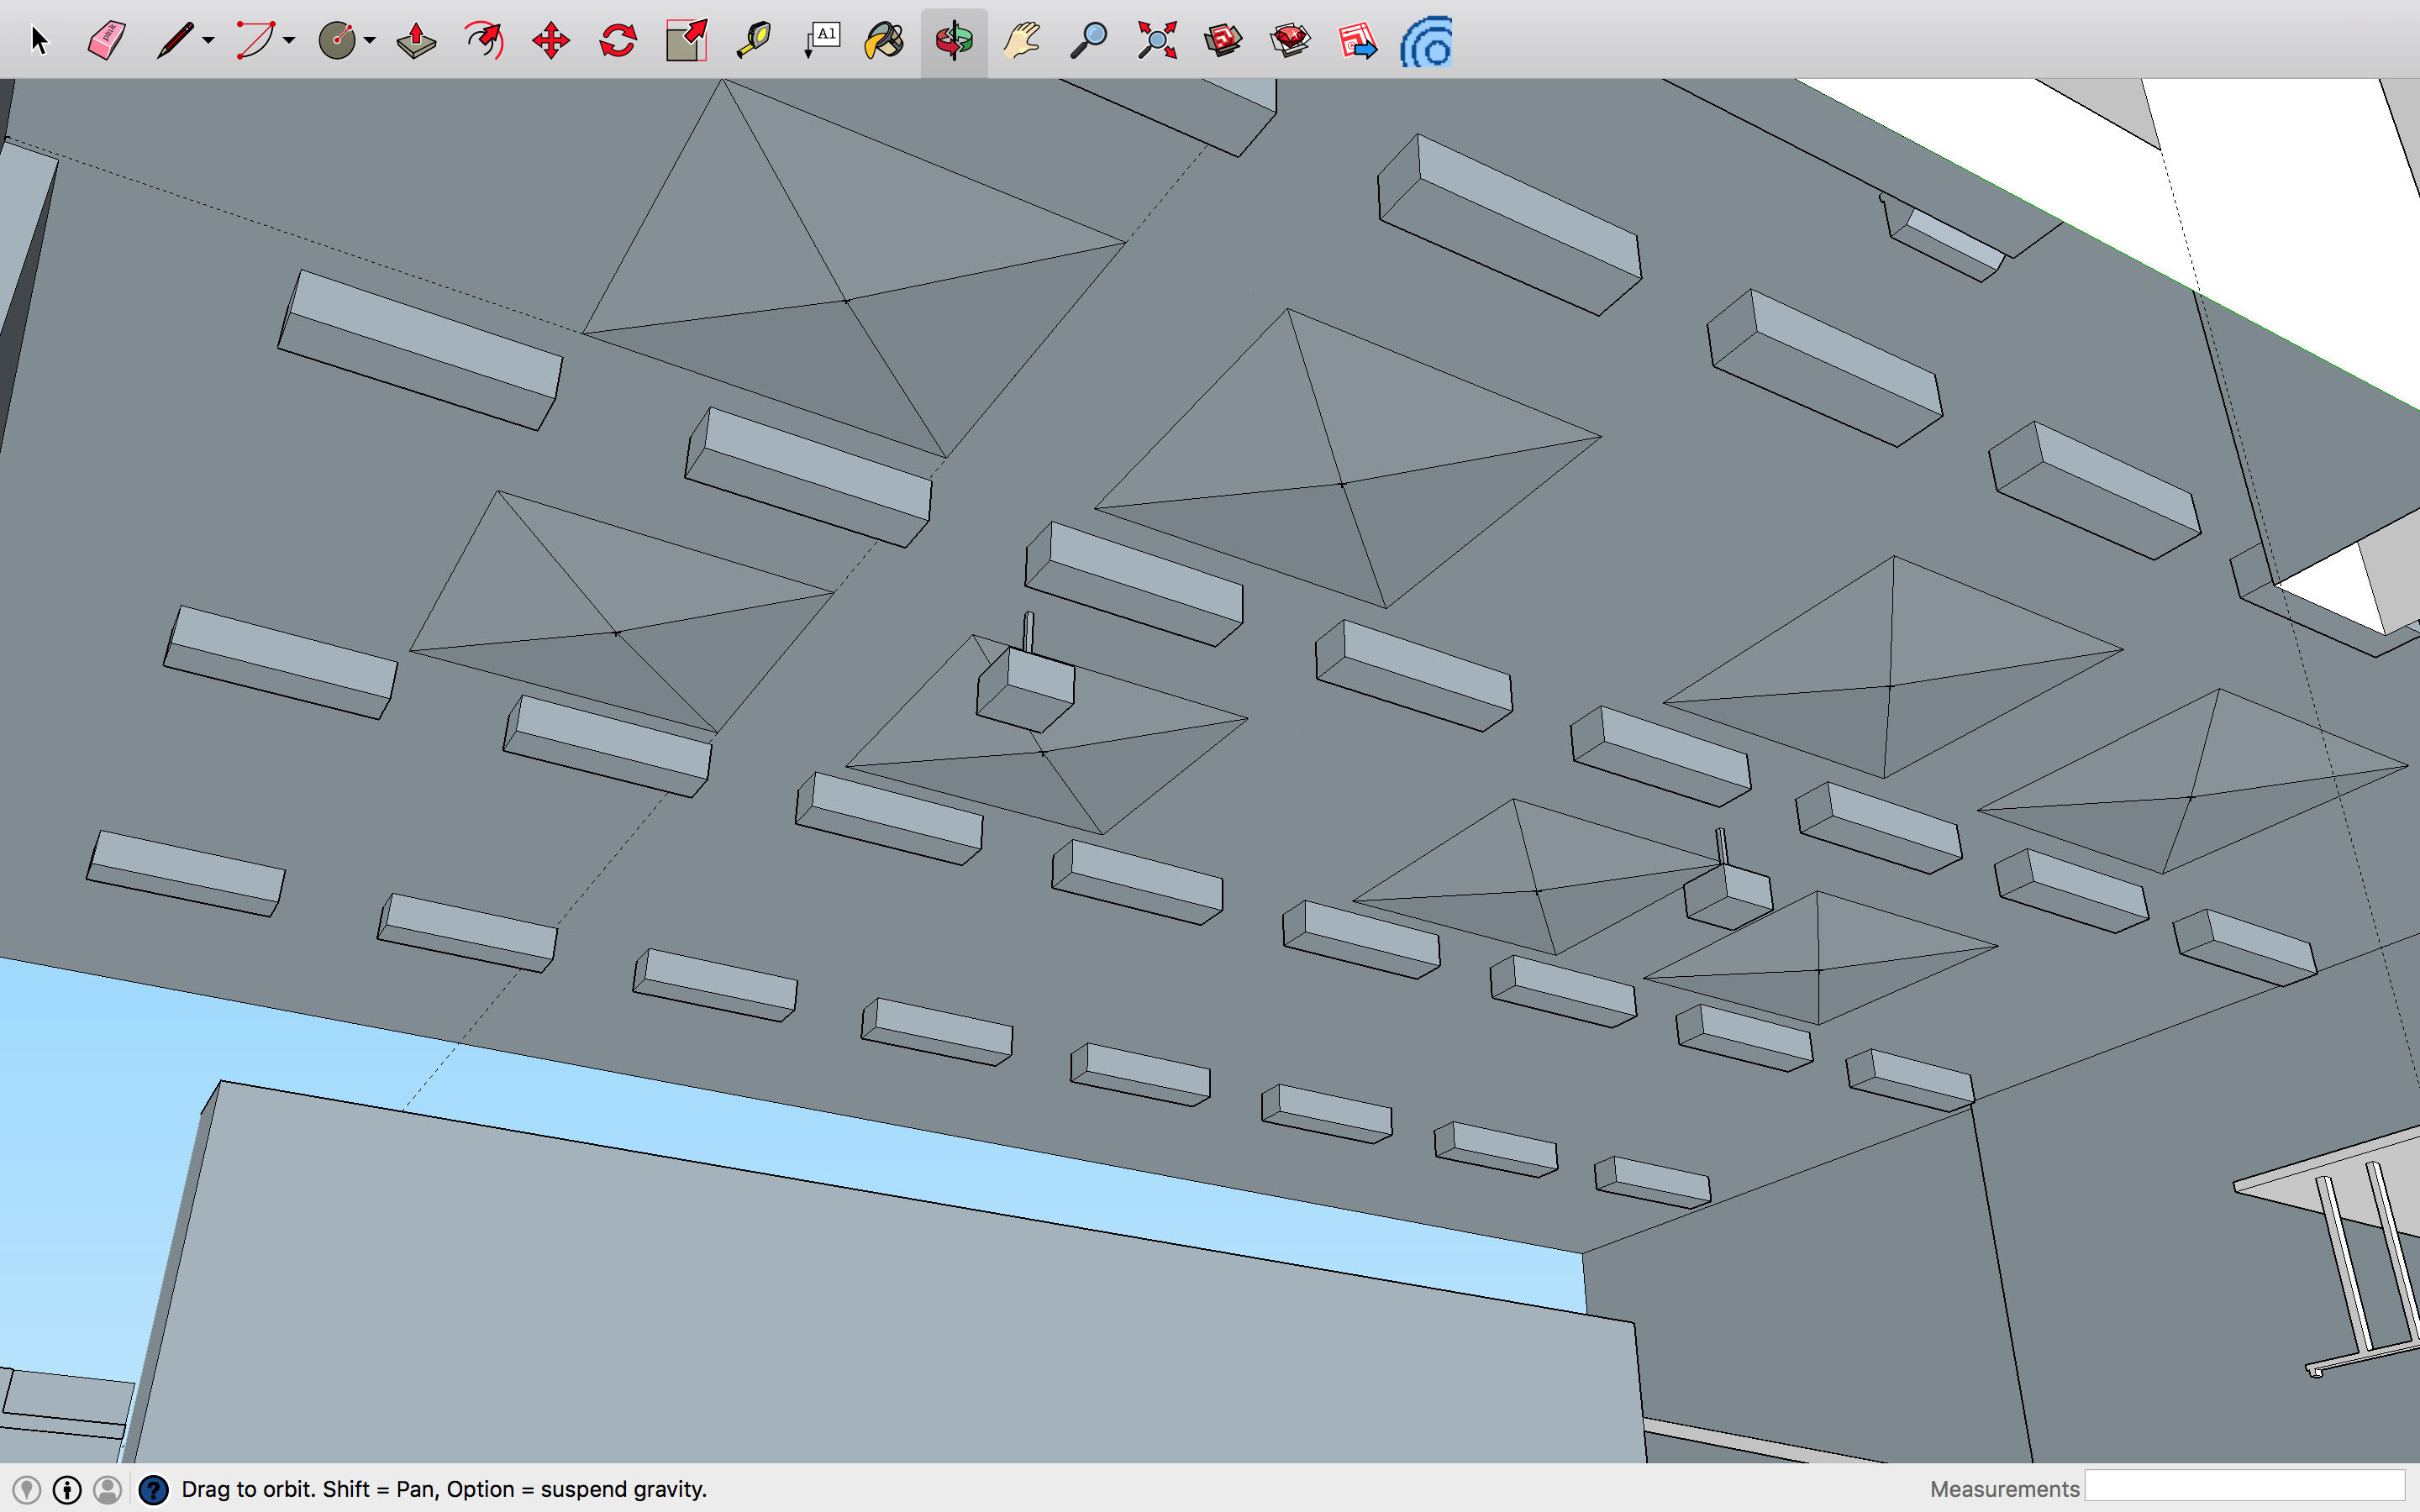
\includegraphics[scale = 0.3]{Sections/Implementation/Modelling/images/realVsSku/roofSku.png}
				\center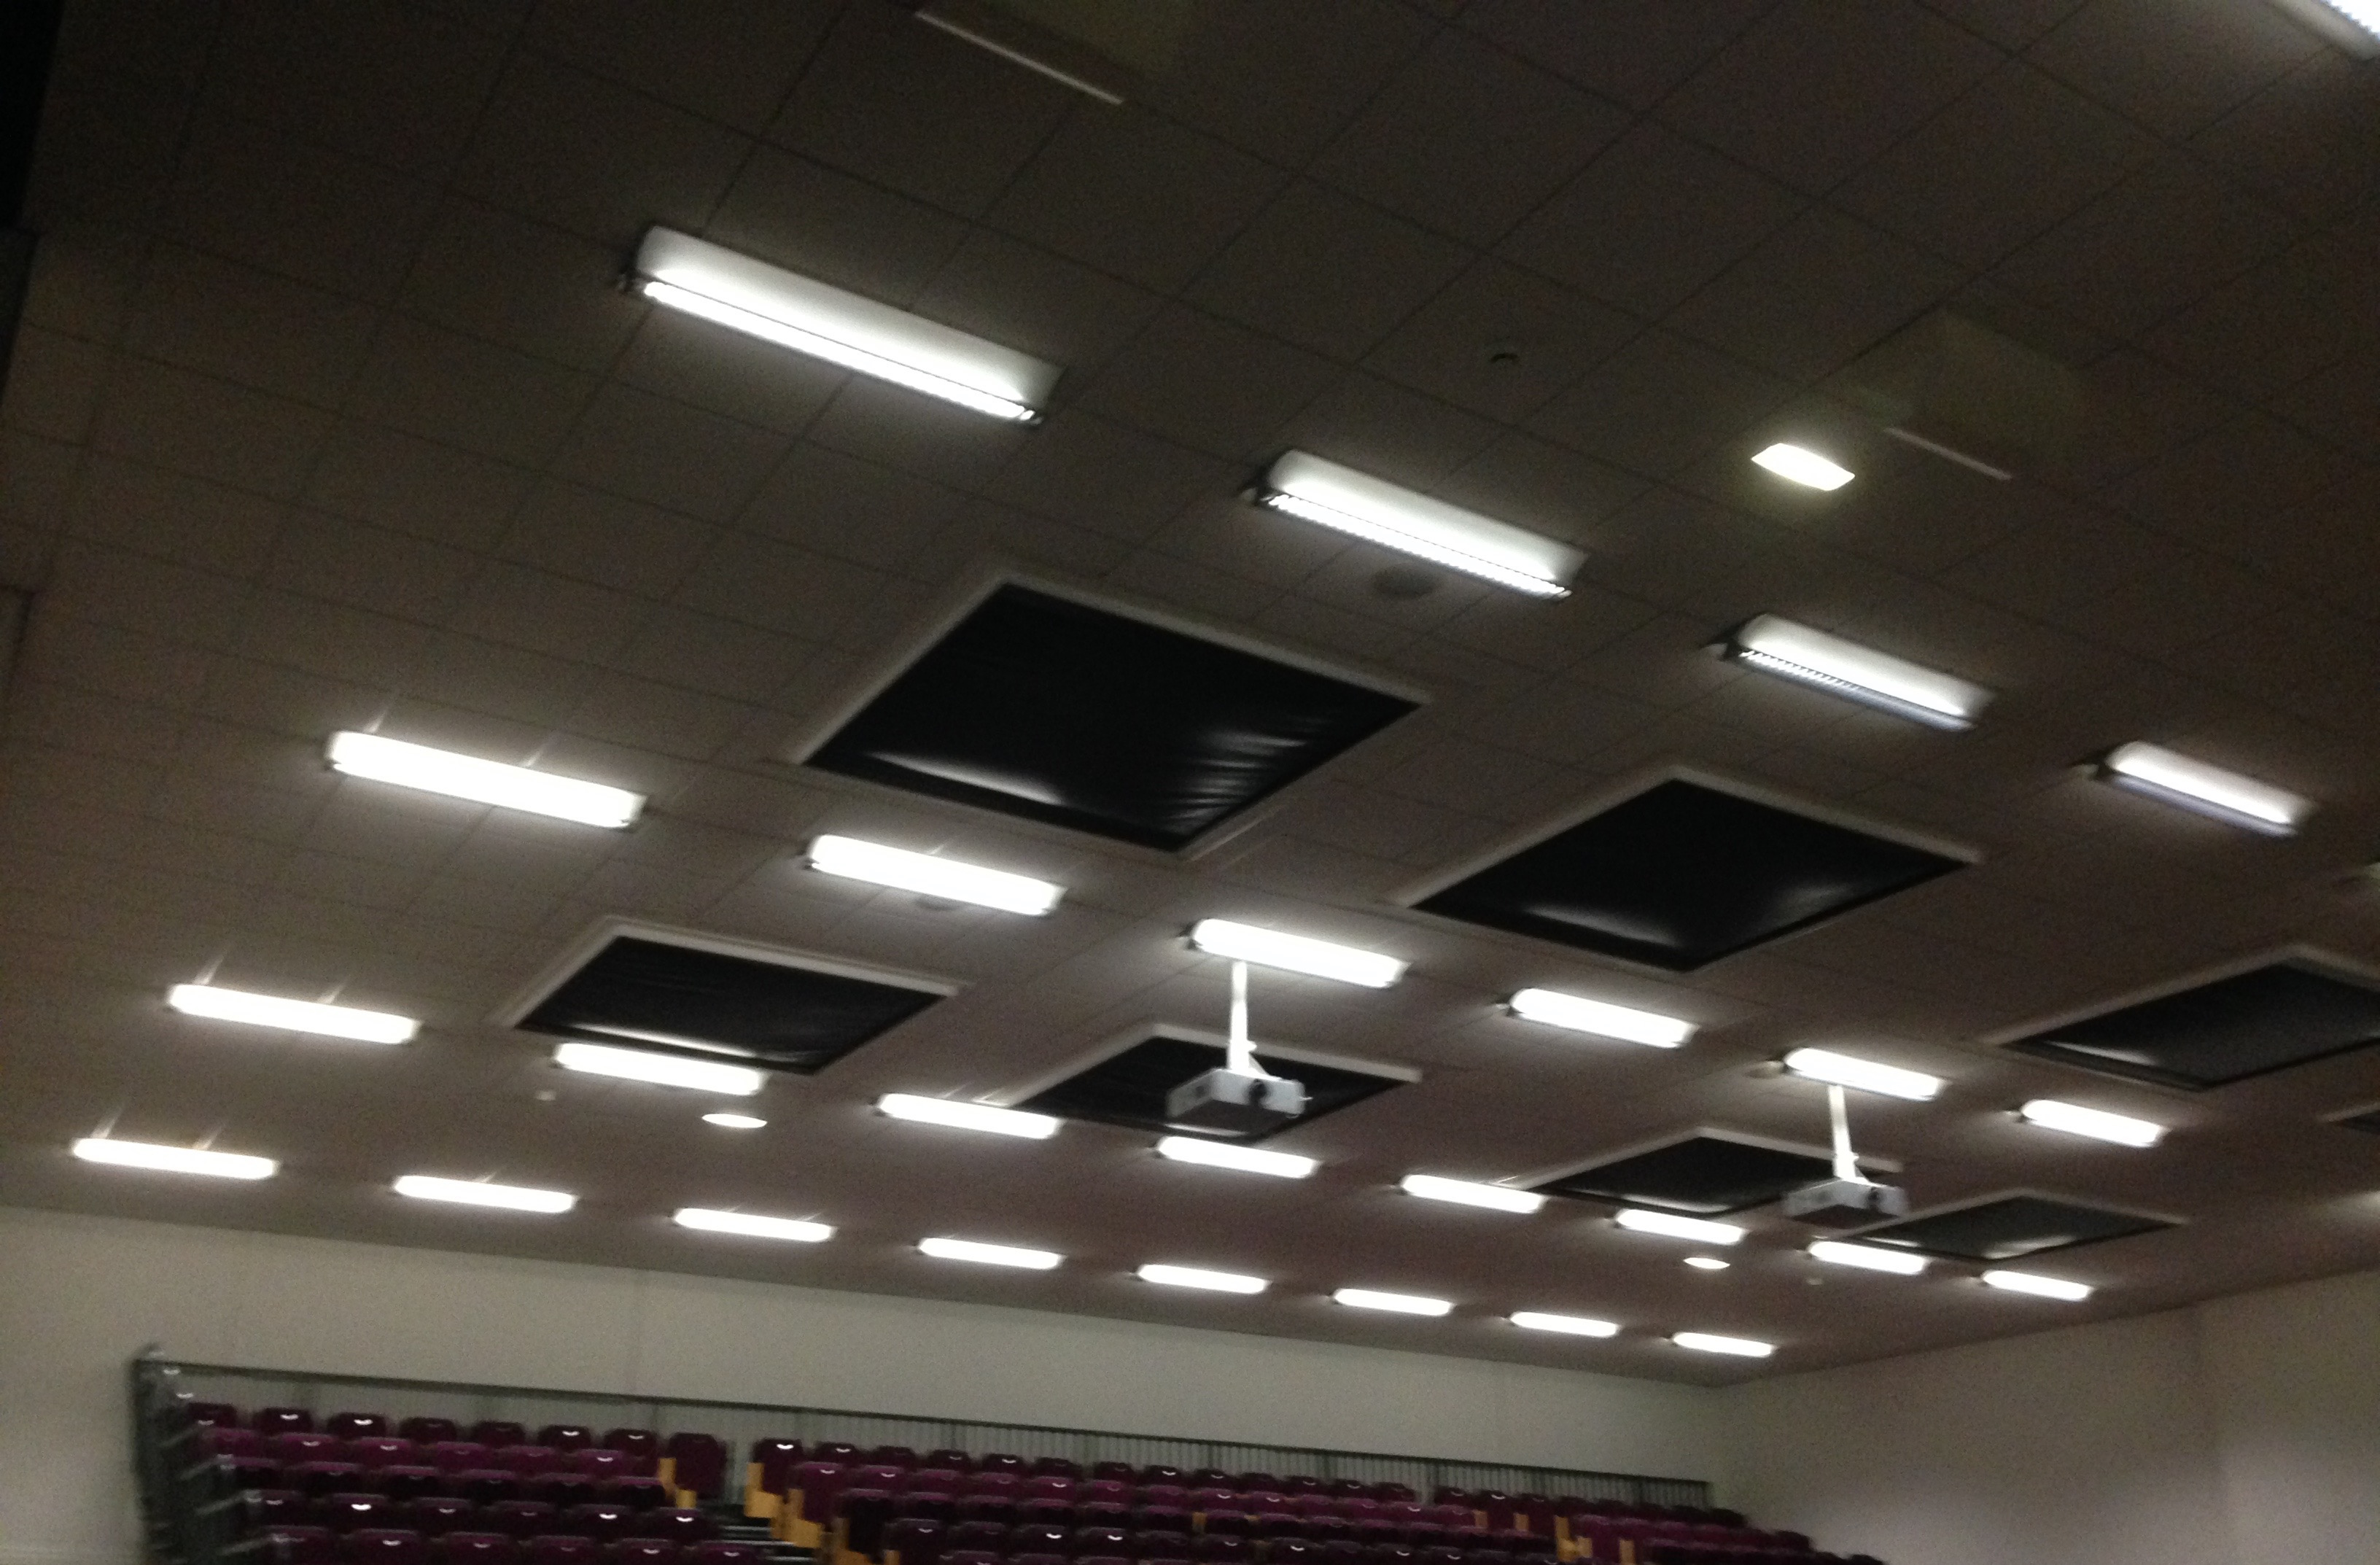
\includegraphics[scale = 0.13]{Sections/Implementation/Modelling/images/HHroof.jpg}
				\caption{Comparison of the final simplified model and a picture of the real Hendrix Hall}
				\label{simpleSurfacesRoom}
			\end{figure}

\end{document}